% !Mode:: "TeX:UTF-8"

\documentclass{zjutthesis}

\graphicspath{{figures/}}  % 定义所有的eps文件在 figures 子目录下
\begin{document}           % 开始全文

%论文题目:{中文}
\zjuttitle{基于内存数据库的大数据应用系统的设计与实现}
%作者:{中文姓名}{学号}
\zjutauthor{陈佳鹏}{20092663503}
%指导教师:{导师中文名}
\zjutmentor{陈~~~~波}
%个人信息:{毕业年份}{专业名称}
\zjutinfo{2013}{软件工程}
%学院信息:{学院中文}
\zjutcollege{计算机科学与技术学院}
%日期:{提交日期}
\zjutdate{2013年06月}

% !Mode:: "TeX:UTF-8"
%%============================================================
%% 中文封面
\thispagestyle{empty}
\pdfbookmark[-1]{\zjuttitlec}{zjutreportcover}
\phantomsection \label{zjutreportcover}
\vspace*{-2.5mm}
% 校名
\begin{center}
   
\includegraphics[width=98.40mm]{figures/zjut}
\end{center}
\vspace*{9.66mm}
\centerline{\songti\yihao{\reporttitle}}
\vspace*{10.0mm}
\centerline{\heiti\xiaoer\textbf{(\zjutgrade\ 届)}}
\vspace*{8.5mm}
% 校徽
\begin{center}
  
\includegraphics[width=27.3mm]{figures/zjutlogo}
\end{center}

\vspace*{0.0mm}
\renewcommand{\arraystretch}{1.0}
\hspace*{7.4mm}
{\songti\erhao{论文题目}}
\hspace{6mm}
\begin{minipage}[t]{95mm}
    \linespread{1.1}{\songti\xiaoer\uline{\zjuttitlec}}
\end{minipage}
\vspace*{9mm}
\begin{center}
    \setlength{\arrayrulewidth}{0.5pt}
    {\songti\sihao
        \renewcommand{\arraystretch}{1.4}
        \begin{tabular}{lc}
            作者姓名 \qquad &  \zjutauthornamec \\ \cline{2-2}
            指导教师\qquad &  \zjutmentorc\\ \cline{2-2}
            \\
            学科(专业)\qquad &  \zjutmajor \\ \cline{2-2}
            所在学院\qquad &  \zjutcollegec \\ \cline{2-2}\cline{2-2}
            提交日期\qquad & \zjutsubmitteddatee \\ \cline{2-2}
        \end{tabular}
    }
\end{center}

      % 封面

\frontmatter

\pagenumbering{Roman}
% !Mode:: "TeX:UTF-8"
%% 中文摘要
\begin{abstractc}
随着互联网的高速发展,各种大数据类型的应用层出不穷。低延迟I/O等高需求的条件对传统的磁盘数据库产生了很大冲击。内存数据库是最近很热门的技术,它将数据完全放在内存中,而传统的硬盘只用做数据库的持久化备份,使得应用程序对数据有极高的处理速度。

本文基于Redis及SQLite等开源数据库,实现了一个大数据的应用系统,重点对Redis底层数据结构的设计原理及方法进行了分析。使用Python语言编写了主要功能的模块,其中GUI部分基于扩展库PyQt4开发。为方便用户使用,本系统在Redis原命令的基础上实现了一些基础的SQL操作(Create,Select 等),并能够在GUI中显示相应的操作结果。在性能测试方面,重点对数据读取性能与热门的关系型数据库MySQL(5.5)进行了对比,比较了两者在读写速度上的差异。

实验结果表明,本系统实现了内存数据库的基本操作。与磁盘数据库相比,在读写性能上有较大的提高,可以满足数据挖掘大数据应用的需求。


% 摘要内容,小四号宋体,段前段后0磅,1.5倍间距。500字左右。每段开头空两格,标点符号占一格。中文摘要应表达毕业设计工作的核心内容,简短明了。
% 首先,摘要应当要素齐全。即一篇摘要应当包含如下要素:
% 1.目的—即从事该项研究开发的理由与背景或所涉及的主题范围;
% 2.方法—即所用的原理﹑理论﹑开发工具,关键技术解决方法等;
% 3.结果—即研究开发工作的结果﹑数据﹑效果﹑性能等;
% 4.结论—即对结果的分析﹑评价等。
% 其次,摘要应当客观﹑如实地反映论文的内容。
% 第三,采用第三人称写法。由于摘要将直接被检索类二次文献采用,脱离原文独立存在,所以摘要一律采用第三人称写法。

\keywordsc{Redis,内存数据库,SQLite,备份恢复}
\end{abstractc}
     % 中文摘要
% !Mode:: "TeX:UTF-8"
%% 英文摘要
\begin{abstracte}
    
Externally pressurized gas bearing has been widely used in the field of aviation,
semiconductor, weave, and measurement apparatus because of its advantage of high accuracy,
little friction, low heat distortion, long life-span, and no pollution.
In this \textit{thesis}, based on the domestic and overseas researching\ldots\ldots

\keywordse{~~Keyword 1,~~Keyword 2,~~Keyword 3}
\end{abstracte}
     % English Abstract

%%%%%%%%%% 目录 %%%%%%%%%%
% \defaultfont TODO format 中定义的fix
% \clearpage{\pagestyle{empty}\cleardoublepage}
% \titleformat{\chapter}{\centering\hei\sanhao\bfseries}{\chaptername}{2em}{} %设置目录两字的格式

\tableofcontents           % 中文目录
\listoffigures             % 图目录
\listoftables              % 表目录

% \defaultfont\sloppy\raggedbottom
% \titleformat{\chapter}{\centering\hei\xiaoer\bfseries}{\chaptername}{2em}{} %恢复chapter标题格式要求

%%%%%%%%%% 正文 %%%%%%%%%%
\mainmatter
% \makeatletter


%%% 第一章 绪论 %%%
% 1.1	字体标题(2级标题,小三,宋体,加粗,段前12磅,段后6磅,1.5倍行距)	1
% 1.2	图表说明	1
% 1.3	公式	2
% 1.4	本文的主要工作	2
% 1.5	本文的组织结构	2
% 1.6	本章小结	3

\chapter{绪论}
\section{课题研究背景}
1969年,埃德加•弗兰克•科德(Edgar Frank Codd)发表了一篇划时代的论文,首次提出关系数据模型的概念。但可惜的是,刊登论文的“IBM Research Report”只是IBM公司的内部刊物,因此论文反响平平。1970年,他再次在刊物《Communication of the ACM》上发表了题为“A Relational Model of Data for Large Shared Data banks”(大型共享数据库的关系模型)的论文,终于引起了大家的关注。

科德所提出的关系数据模型的概念成为了现今关系型数据库的基础。当时的关系型数据库由于硬件性能低劣、处理速度过慢而迟迟没有得到实际应用。但之后随着硬件性能的提升,加之使用简单、性能优越等优点,关系型数据库得到了广泛的应用。

但是现如今随着互联网的不断发展,各种类型的应用层出不穷,所以导致在这个云计算的时代,对技术提出了更多的需求,传统关系型数据库面临很多问题,主要体现在下面这四个方面:
\begin{enumerate}[label=(\arabic*)]
\item{低延迟的读写速度:应用快速地反应能极大地提升用户的满意度}
\item{支撑海量的数据和流量:对于搜索这样大型应用而言,需要利用PB级别的数据和能应对百万级的流量}
\item{大规模集群的管理:系统管理员希望分布式应用能更简单的部署和管理}
\item{庞大运营成本的考量:IT经理们希望在硬件成本、软件成本和人力成本能够有大幅度地降低}
\end{enumerate}

虽然关系型数据库已经在业界的数据存储方面占据不可动摇的地位,但是由于其天生的几个限制,使其很难满足下面的这几个需求:
\begin{enumerate}[label=(\arabic*)]
\item{扩展困难:当需要表与表之间Join操作时,数据库就不能很好的进行扩展}
\item{读写速度慢:当数据量达到较大规模的时候,很容易发生死锁的问题,直接导致读写速度急剧下降的问题}
\item{成本高:企业级数据库的License价格惊人,且随着系统的规模而不断上升}
\item{有限的支撑容量:现有关系型解决方案还无法支撑Google这样海量的数据存储}
\end{enumerate}

而因此思想诞生的内存数据库(MMDB)对数据访问读取有着很高的效率,对于一些需要
在严格要求的时间段内完成事务请求
的实时应用系统,和需要支持大量并发访问的高性能事务处理平台来而言,它都是一个很不错的选择。

\section{研究与应用现状}
国内外相关人员经过长年的研究,设计并实现了多种内存数据库的
模型及商用或开源的产品。商用MMDB的代表产品有AltiBase、Timesten,SAP HANA等,开源
产品主要有FastDB、SQLite、Redis等,下文对一些数据库做简单的介绍:

\subsection{Oracle TimesTen}
Oracle TimesTen内存数据库是一个功能全面的关系型内存数据库,旨在通过在应用层的运行,加速处理响应时间和关键任务型应用所需的高吞吐量。从某种角度上来看,TimesTen也是一种Cache机制,是磁盘数据库的‘Cache’,通过物理内存中的数据存储区的直接操作,减少了到磁盘间的I/O交互。TimesTen中的这个Ten据说就是指速度能达到基于磁盘的RDBMS10倍。

\subsection{SAP HANA}
SAP HANA是一款面向数据源的、灵活、多用途的内存应用设备,整合了基于硬件优化的SAP软件模块,通过SAP主要硬件合作伙伴提供给客户。SAP HANA提供灵活、节约、高效、实时的方法管理海量数据。利用HANA,企业可以不必运行多个数据仓库、运营和分析系统,从而削减相关的硬件和维护成本。SAPHANA将在内存技术基础上,为新的创新应用程序奠定技术基础,支持更高效的业务应用程序,如:计划、预测、运营绩效和模拟解决方案。

\subsection{Redis}
Redis是一个高性能的key-value存储系统。和Memcached类似,它支持存储的value类型相对更多,包括string(字符串)、list(链表)、set(集合)和zset(有序集合)。这些数据类型都支持push/pop、add/remove及取交集并集和差集及更丰富的操作,而且这些操作都是原子性的。在此基础上,redis支持各种不同方式的排序。与memcached一样,为了保证效率,数据都是缓存在内存中。区别的是redis会周期性的把更新的数据写入磁盘或者把修改操作写入追加的记录文件,并且在此基础上实现了master-slave(主从)同步。

\section{本文主要工作}
本文的主要工作是在详细分析内存数据库系统需求的基础上,对其详细设计和具体实现以及之后的相关测试进行阐述。

\section{本文的组织结构}
本文共分为八章,以内存数据库为背景,研究讨论了基于Redis并支持SQL架构的内存数据库,详细阐述了如何利用该框架技术对系统的模块进行设计与实现,各章内容如下:

第一章,介绍了课题研究的背景,国内外相关领域的研究及应用,课题研究的主要任务和本文的主要工作。

第二章,详细介绍了内存数据库应用系统开发的方法与技术,为系统的后续开发做准备。

第三章,重点介绍了内存数据库应用系统的需求。

第四章,具体介绍了内存数据库应用系统的概要设计。

第五章,详细介绍了内存数据库应用系统的详细设计。其内容包括开发规范的确定、系统所采用框架的整合设计、功能模块的详细设计和系统性能要求的详细设计。

第六章,着重阐述了内存数据库应用系统的具体实现,针对第五章提出的详细设计要求,在本章给出系统的技术实现,具体包括系统框架整合实现、功能性能要求实现和系统功能模块实现。

第七章,系统测试与系统使用说明。

第八章,对系统开发进行总结并提出下一步工作。


%%% 第二章 方法与技术 %%%
% 2.1	Spring框架简介	4
% 2.1.1	Spring的控制反转(IoC)(3级标题,四号,宋体,加粗,段前6磅,1.5倍行距,建议不使用四级或更高级别目录、标题)	4
% 2.1.2	面向切面编程(AOP)	4
% 2.1	Hibernate框架	4
% 2.2	AJAX	5
% 2.3	Ext框架	5
% 2.4	DWR技术	5
% 2.5	开发环境	5
% 2.5.1	服务器端环境要求	5
% 2.5.2	客户端环境要求	5
% 2.6	主要开发语言	6
% 2.7	开发原则	6
% 2.8	本章小结	6

\chapter{方法与技术}
本系统采用了后端Redis配合SQLite的C语言接口,前端GUI使用PyQT4的架构,实现了支持一些基础SQL语句的内存数据库应用系统,本章将对上述知识进行简要的阐述。

\section{Redis}
Redis是一个开源的使用ANSI C语言编写、支持网络、可基于内存亦可持久化的日志型、Key-Value数据库,并提供多种语言的API。作为Key-value型数据库,Redis也提供了键(Key)和键值(Value)的映射关系。但是,除了常规的数值或字符串,Redis的键值还可以是以下形式之一:

Lists(列表)

Sets(集合)

Sorted sets(有序集合)

Hashes(哈希表)

键值的数据类型决定了该键值支持的操作。Redis支持诸如列表、集合或有序集合的交集、并集、差集等高级原子操作;同时,如果键值的类型是普通数字,Redis则提供自增等原子操作。通常,Redis将数据存储于内存中,或被配置为使用虚拟内存。通过两种方式可以实现数据持久化:使用快照的方式,将内存中的数据不断写入磁盘;或使用类似MySQL的日志方式,记录每次更新的日志。前者性能较高,但是可能会引起一定程度的数据丢失;后者相反。

相比需要依赖磁盘记录每个更新的数据库,基于内存的特性无疑给Redis带来了非常优秀的性能。读写操作之间没有显著的性能差异,如果Redis将数据只存储于内存中。

\section{SQLite}
SQLite是遵守ACID的关系数据库管理系统,它包含在一个相对小的C库中。它是D.RichardHipp创建的公有领域项目。
不像常见的客户端/服务器结构范例,SQLite引擎不是个程序与之通信的独立进程,而是连接到程序中成为它的一个主要部分。所以主要的通信协议是在编程语言内的直接API调用。这在消耗总量、延迟时间和整体简单性上有积极的作用。整个数据库(定义、表、索引和数据本身)都在宿主主机上存储在一个单一的文件中。它的简单的设计是通过在开始一个事务的时候锁定整个数据文件而完成的。

\section{Python}
Python是个成功的脚本语言。它最初由Guido van Rossum开发,在1991年第一次发布。Python由ABC和Haskell语言所启发。Python是一个高级的、通用的、跨平台、解释型的语言,一些人更倾向于称之为动态语言。它很易学,Python是一种简约的语言。它的最明显的一个特征是,不使用分号或括号,Python使用缩进。最近的版本是2.7(3.2),2011年二月发布。现在,Python由来自世界各地的庞大的志愿者维护。Python是那些想要学习编程的人的理想的入门语言,它支持多种编程模式,它不强制程序员使用特定的模式。Python支持面向对象和面向过程编程,也有限的支持函数式编程。

\section{PyQT4}
PyQT是一个生成图形应用程序的工具包。是python语言和成功的Qt库的绑定。Qt库是这个世界上最强大的库之一,PyQT作为一组python的模块来实现。它包含了超过300个类,将近6000个函数和方法。它是一个多平台的工具包,可以在所有的主流操作系统上运行,包括Unic,Windows和Mac。PyQT采用双协议,开发者可以在GPL和商业授权中选择。以前的版本中,GPL版本只存在于Unic上。从PyQT4开始,GPL协议支持所有的平台。QtCore模块包含了核心的非图形功能,这个模块被用来实现时间,文件和目录,不同的数据格式,流,互联网地址,mime类型,线程或进程等等。QtGui模块包含了图形组件和类的描述,包括例如按钮,窗口,状态栏,滑块,位图,颜色,字体等等。

QtCore模块包含了核心的非图形功能,这个模块被用来实现时间,文件和目录,不同的数据格式,流,互联网地址,mime类型,线程或进程等等。

QtGui模块包含了图形组件和类的描述,包括例如按钮,窗口,状态栏,滑块,位图,颜色,字体等等。

QtNetwork模块包含了网络编程所需的类,这些类可以用来实现TCP/IP和UDP的客户端/服务器程序,使得网络编程更加简单更加可移植。

QtXml模块提供了处理xml文件的类,这个模块包含了SAX和DOM APIs的实现。

QtSvg模块包含了显示SVG文件目录的类。Scalable Vector Graphics (SVG)是一种利用XML来描述二维图形和图形应用的的语言。

QtOpenGL模块用来通过OpenGL库来渲染3D和2D图形,这个模块实现了Qt GUI库和OpenGL库的无缝集合。

QtSql模块提供了处理数据库的类。

\section{本章小结}
本章以本系统开发的相关理论及技术为基础,介绍系统开发过程中需要了解和掌握的方法和技术,详细阐述了Redis,SQLite,PyQT4d等相关技术。


\chapter{需求分析}
% 3.1	系统简介	7
% 3.1.1	项目类别和申报类型	7
% 3.1.2	系统使用对象	7
% 3.1.3	功能概述	7
% 3.2	系统的整体框架	7
% 3.3	本章小结	8

\section{系统简介}
由于Redis本身Key-Value的特性,它可以在很多Web应用场景上发挥巨大的功效,下文列举了几个常见的应用场景:
\begin{enumerate}[label=(\arabic*)]
\item{在主页中显示最新的项目列表。
由于Redis使用的是常驻内存的缓存,速度非常快。LPUSH用来插入一个内容ID,作为关键字存储在列表头部。LTRIM用来限制列表中的项目数最多为5000。如果用户需要的检索的数据量超越这个缓存容量,这时才需要把请求发送到数据库。}

\item{排行榜及相关问题。
排行榜按照得分进行排序,ZADD命令可以直接实现这个功能,而ZREVRANGE命令可以用来按照得分来获取前N名的用户,ZRANK可以用来获取用户排名}

\item{按照用户投票和时间排序。
这就像Reddit的排行榜,得分会随着时间变化。LPUSH和LTRIM命令结合运用,把文章添加到一个列表中。一项后台任务用来获取列表,并重新计算列表的排序,ZADD命令用来按照新的顺序填充生成列表。列表可以实现非常快速的检索,即使是负载很重的站点。}

\item{计数。进行各种数据统计的用途是非常广泛的,比如想知道什么时候封锁一个IP地址。INCRBY命令让这些变得很容易,通过原子递增保持计数;GETSET用来重置计数器;过期属性用来确认一个关键字什么时候应该删除。}

\item{队列。在当前的编程中队列随处可见。除了push和pop类型的命令之外,Redis还有阻塞队列的命令,能够让一个程序在执行时被另一个程序添加到队列。你也可以做些更有趣的事情,比如一个旋转更新的RSS feed队列。}

\item{缓存。
Redis缓存使用的方式与memcached相同。
网络应用不能无休止地进行模型的战争,看看这些Redis的原语命令,尽管简单但功能强大,把它们加以组合,所能完成的就更无法想象。当然,你可以专门编写代码来完成所有这些操作,但Redis实现起来显然更为轻松。}
\end{enumerate}

但是,Redis并非是传统的关系型数据库,无法支持SQL语句解析,所以本系统在这基础上配合采用了SQLite的接口,同时为Redis新增加了一个基于SQLite的“sql”命令。至此,可以通过sql命令来进行数据库的表操作,表中的所有数据完全存储在内存中,此外,根据Redis.conf的配置,可以设置表中数据库每次保存到硬盘的间隔,这样做可以保证数据的正确性,防止出现可能的断电宕机使数据丢失的情况。

综上所述,内存数据库应用系统可以同时通过Redis的命令来直接操作“Key-Value”的数据集,或者通过附加的“sql”命令来操作传统的关系型数据库中的表集合,两者都放在内存中。

\section{系统框架}
整个系统的框架主要分两部分:Server(服务器端)和Client(客户端),两者通过套接字来进行交互,数据的格式必须满足Redis的协议:
\begin{verbatim}
*<参数数量>\r\n$<第1个参数字节数>\r\n<参数数据>\r\n...$<第N个参数字节数>\r\n<参数数据>\r\n
例如:*3\r\n$3\r\nSET\r\n$5\r\nmykey\r\n$7\r\nmyvalue\r\n
\end{verbatim}

%%% 架构图 %%%
整个系统的框架图如图~\ref{fig:Network}~所示。
\begin{figure}[H]
\centering
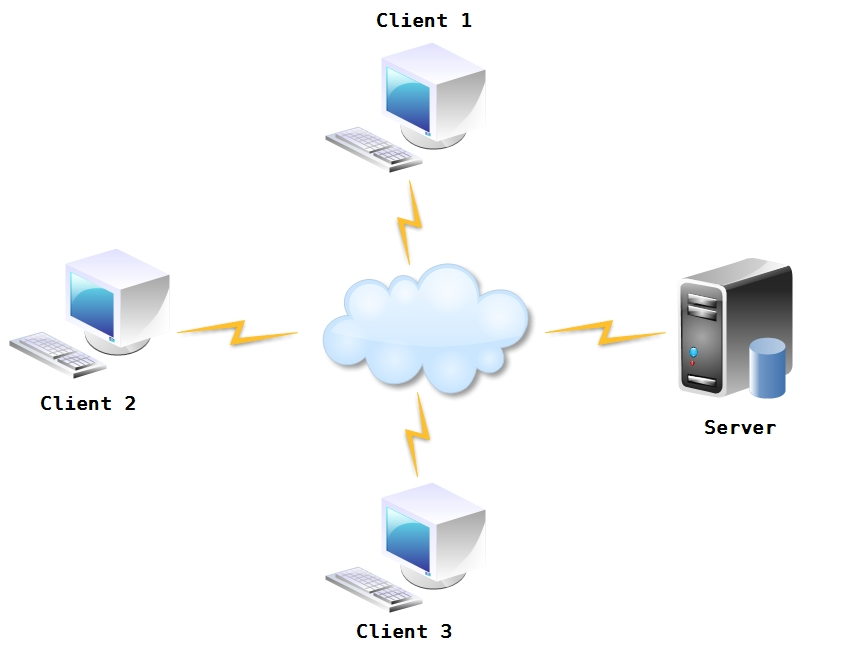
\includegraphics[width=0.8\textwidth]{Network}
\caption{系统框架图}\label{fig:Network}
\vspace{\baselineskip} %表示图与正文空一行
\end{figure}

\subsection{服务器端}
这里的服务器端就是Redis本身的Server, 除了维持服务器状态之外, 最重要的就是将Redis的各个功能模块组合起来。
简单而言,服务器端就是整个系统的“心脏”,它维护着各个模块,保证每个模块稳定健康的运行,如图~\ref{fig:Redis-Server}~所示。
\begin{figure}[H]
\centering
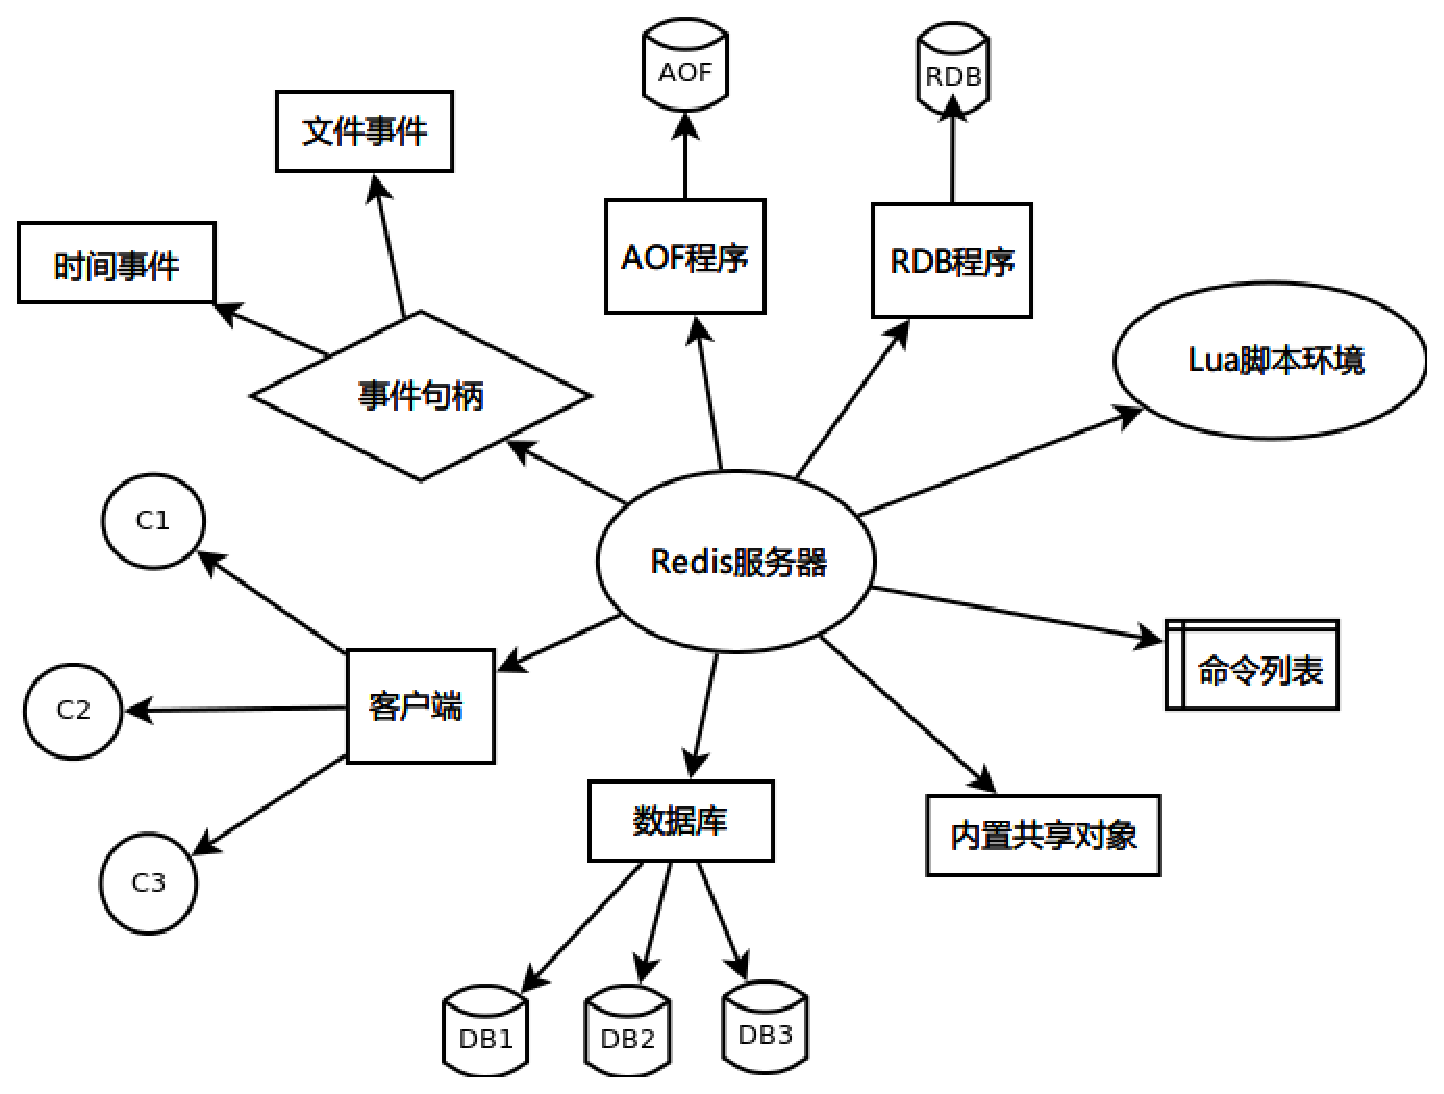
\includegraphics[width=0.8\textwidth]{Redis-Server}
\caption{Redis Server架构图}\label{fig:Redis-Server}
\vspace{\baselineskip} %表示图与正文空一行
\end{figure}

\subsection{客户端}
客户端的作用就是与服务器端进行交互,通过指令来操作控制服务器端。两者之间的交互过程如下:客户端向服务器发送命令,服务器接受命令然后将命令传给命令执行器,执行器执行给定命令的实现函数,执行完成之后,将结果保存在缓存,最后回传给客户端。同时,服务器端可以接受来自多个客户端发来的命令请求。

\section{本章小结}
本章对内存数据库应用系统需求进行了充分的分析,明确了系统框架、大致功能结构等问题,为后续系统设计打下了基础。


%%% 第四章 项目中期检查系统概要设计	%%% 
\chapter{概要设计}
% 4.1	系统业务流程	9
% 4.1.1	业务流程	9
% 4.2	系统功能结构	10
% 4.3	系统架构设计	11
% 4.4	系统数据库设计	11
% 4.5	本章小结	15
\section{系统业务流程}
\subsection{业务流程}
从客户端发送命令请求, 到命令被服务器处理、并将结果返回客户端, 整个过程有以下步骤:
\begin{enumerate}[label=(\arabic*)]
\item{客户端通过套接字向服务器传送命令协议数据。}
\item{服务器通过读事件来处理传入数据,并将数据保存在客户端对应redisClient结构的查询缓存中。}
\item{根据客户端查询缓存中的内容,程序从命令表中查找相应命令的实现函数。}
\item{程序执行命令的实现函数,并将命令的执行结果保存到客户端redisClient结构的回复缓存中,然后为该客户端关联写事件。}
\item{当客户端写事件就绪时,将回复缓存中的命令结果传回给客户端。}
\end{enumerate}

整个流程图如图~\ref{fig:Flow-Chart}~所示。
\begin{figure}[H]
\centering
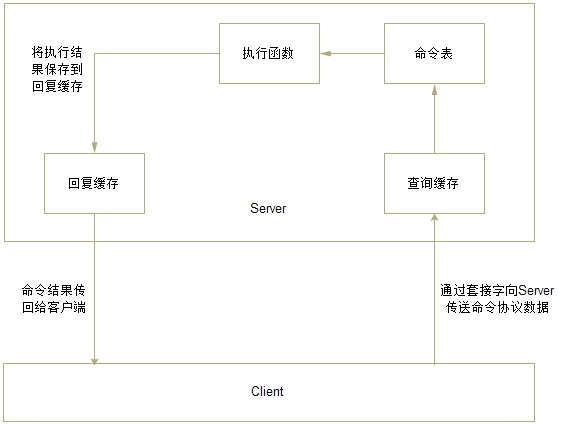
\includegraphics[width=0.7\textwidth]{Flow-Chart}
\caption{Client请求处理图}\label{fig:Flow-Chart}
\vspace{\baselineskip} %表示图与正文空一行
\end{figure}

%%% TODO 业务流程图

服务器启动之后,它便在6379端口(默认端口)监听来自客户端的请求,此时客户端可以连接到某个服务器,然后发送指令请求。如果客户端连接对应的服务器未启动,那客户端发送的命令的请求都会返回错误。

\section{系统功能结构}
%%% TODO 系统功能图 %%%
本系统功能主要分两部分:Redis元命令部分,SQL部分,系统的功能结构如图~\ref{fig:Command}~所示。
\begin{figure}[H]
\centering
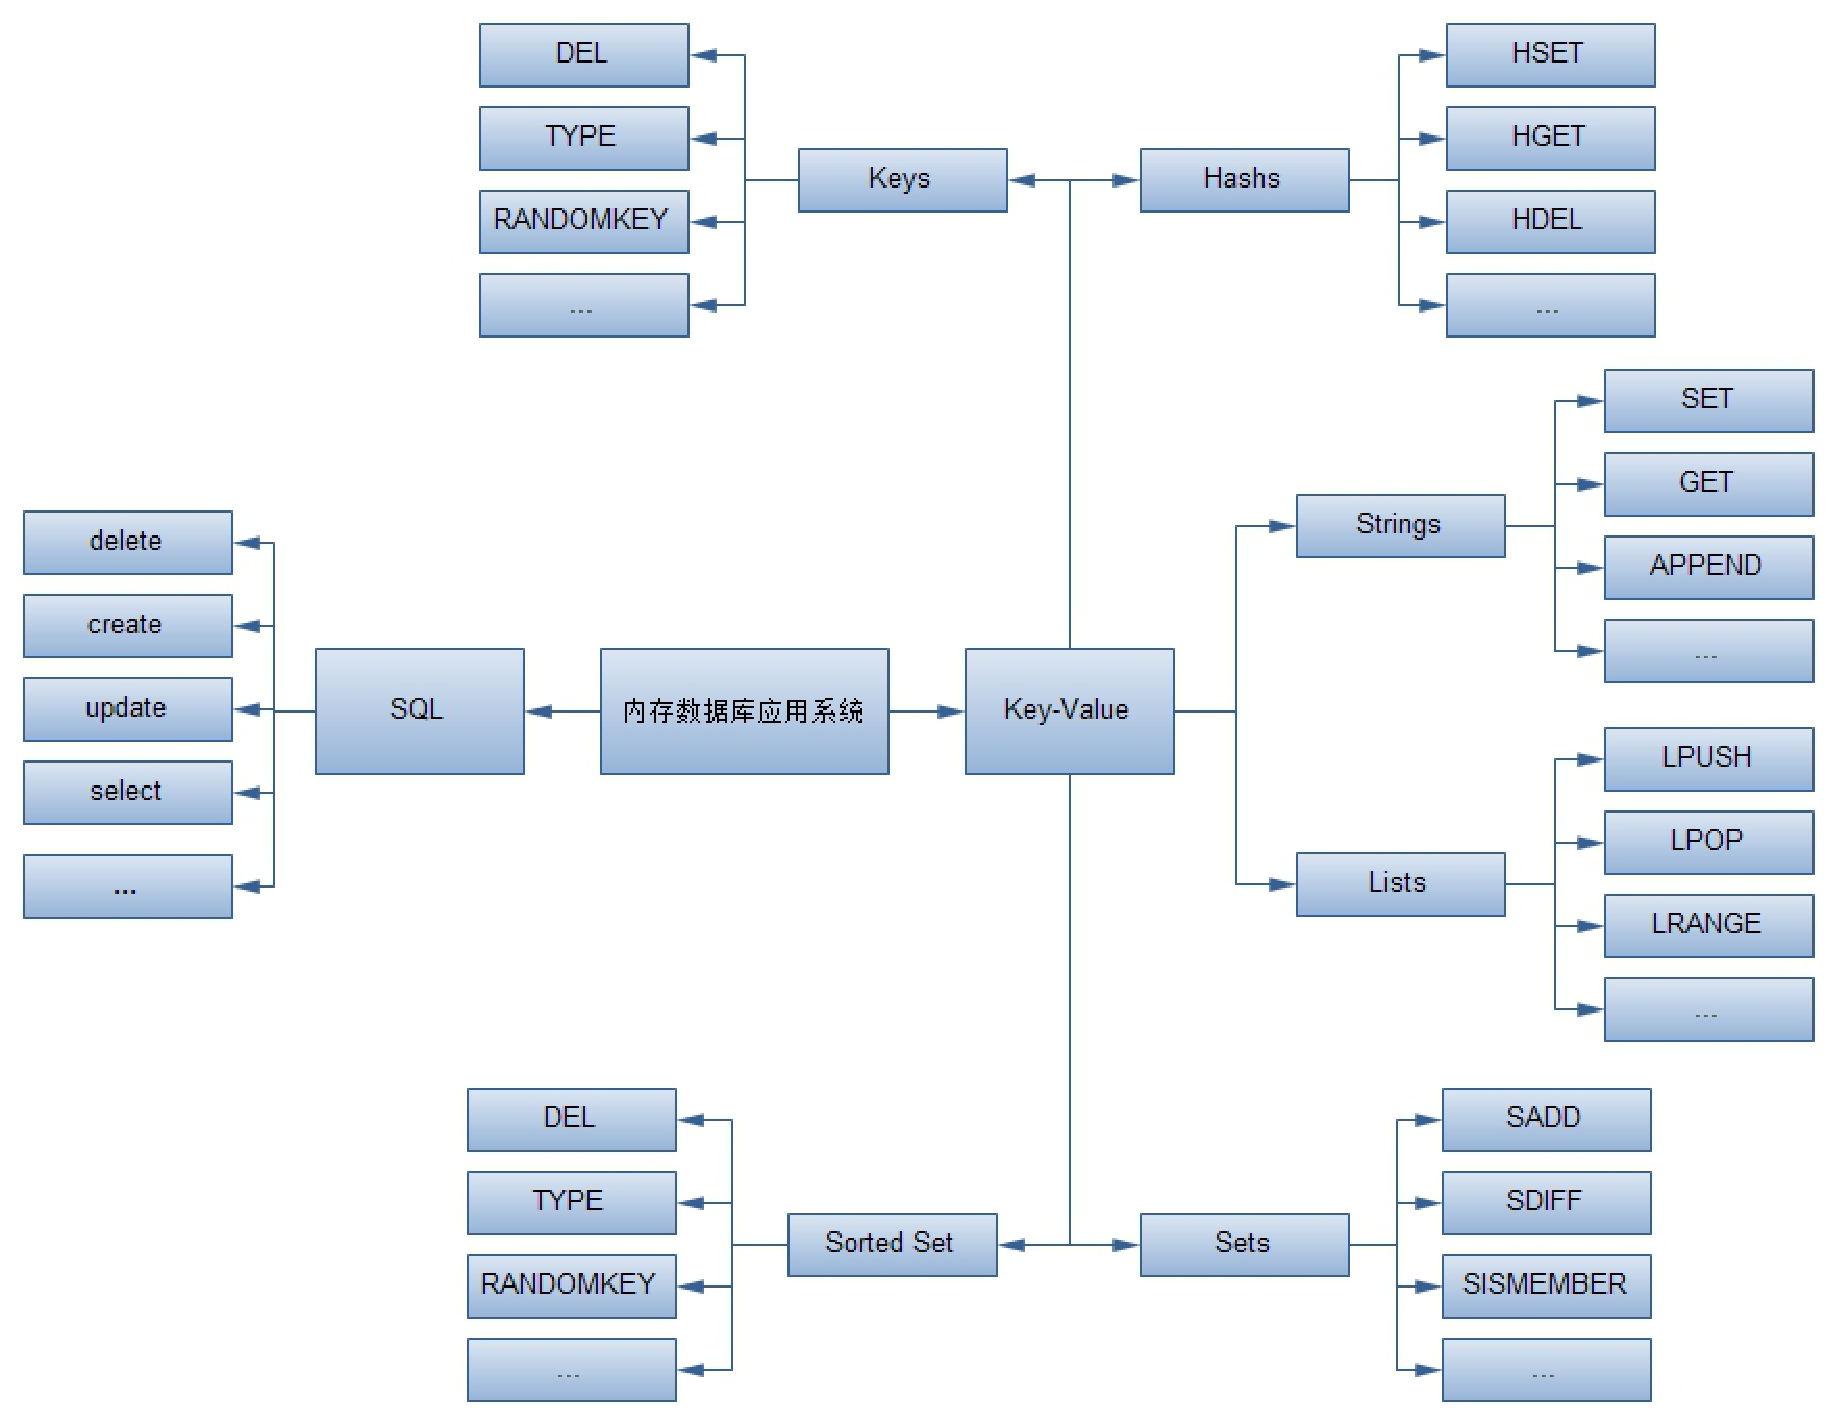
\includegraphics[width=0.9\textwidth]{Command}
\caption{系统功能结构图}\label{fig:Command}
\vspace{\baselineskip} %表示图与正文空一行
\end{figure}

\section{系统架构设计}
%%% TODO 系统的架构图%%%

系统的架构设计如图~\ref{fig:System}~所示。
\begin{figure}[H]
\centering
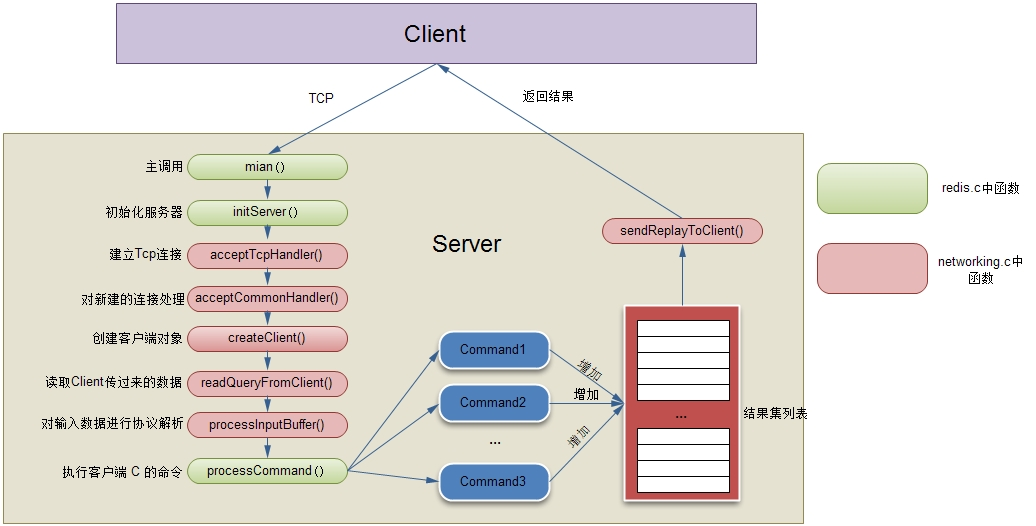
\includegraphics[width=\textwidth]{System}
\caption{系统的架构图}\label{fig:System}
\vspace{\baselineskip} %表示图与正文空一行
\end{figure}

\section{本章小结}
本章主要对内存数据库系统进行了概要设计。首先,对本系统进行了详细的阐述并进行系统架构设计。然后,确定了系统的总体功能结构,概要描述了各个功能模块的详细要求。


%%% 第五章 项目中期检查系统详细设计	 %%%
% 5.1	项目开发规范	16
% 5.1.1	系统目录规划	16
% 5.1.2	命名规则	17
% 5.2	系统功能模块详细设计	17
% 5.3	系统性能优化设计	19
% 5.4	本章小结	19
\chapter{系统详细设计}
\section{项目开发规范}
开发规范在项目的开发过程中具有非常重要的作用,良好的开发规范可以提高软件开发质量,降低开发周期,增强代码的可重用性和易读性,使软件便于维护。

\subsection{系统目录规划}
%%% TODO 系统目录规划表 %%%
系统的目录规划表主要分两个部分:Redis部分和GUI界面部分,如表~\ref{tab:redis-files}~和表~\ref{tab:GUI-files}~所示。

\begin{table}[H]
\centering
\caption{系统目录规划表(Redis部分)}\label{tab:redis-files}
\vspace{0.5em}{\centering\wuhao
\begin{tabular}{|c|c|}
\toprule[1.5pt]
目录 & 名称及说明\\
\midrule[1pt]
表中数据(1,1) & 表中数据(1,2)\\
\bottomrule[1.5pt]
\end{tabular}}
\vspace{\baselineskip}
\end{table}

\begin{table}[H]
\centering
\caption{系统目录规划表(GUI部分)}\label{tab:GUI-files}
\vspace{0.5em}{\centering\wuhao
\begin{tabular}{|c|c|}
\toprule[1.5pt]
目录 & 名称及说明\\
\midrule[1pt]
表中数据(1,1) & 表中数据(1,2)\\
\bottomrule[1.5pt]
\end{tabular}}
\vspace{\baselineskip}
\end{table}

%%% TODO 选择器 %%%
\section{系统功能模块详细设计}
在上文中,图~\ref{fig:Command}~说明了主要的功能模块,包括SQL模块和Redis元命令模块,这两个模块的主要功能就是执
行相关的命令,并返回相应的结果,但是两者的命令都是从同一数据源(GUI)获得的,必须通过“选择器”来确定一条命令是属于SQL模块还是Redis模块,具体设计流程如图~\ref{fig:Selector}~所示。
\begin{figure}[H]
\centering
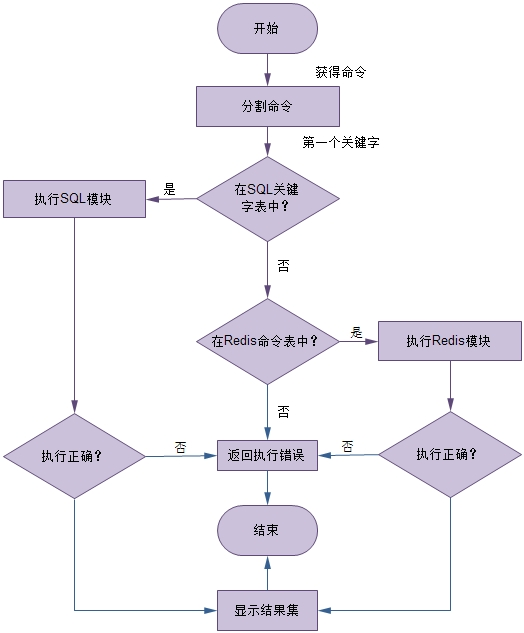
\includegraphics[width=0.9\textwidth]{Selector}
\caption{选择处理模块的流程设计}\label{fig:Selector}
\vspace{\baselineskip} %表示图与正文空一行
\end{figure}

\section{性能优化设计}
\begin{enumerate}[label=(\arabic*)]
\item{根据系统不同需求,修改redis.config中的参数}
\end{enumerate}

\section{本章小结}
本章在第三章、第四章的基础上对系统进行了详细设计。首先,在系统开发之前,对系统的开发规范,包括目录规划进行了规定。重点介绍系统功能模块的详细设计及其流程,紧接着对性能优化等方面进行了设计。

%%% 第六章 项目中期检查系统实现	%%%
\chapter{系统实现}
% 6.1	系统界面实现	20
% 6.2	系统框架整合实现	23
% 6.3	系统功能模块实现	23
% 6.4	本章小结	23

\section{系统界面实现}
本系统中所有的界面均采用PyQT4进行设计,如%%%TODO
所示

\section{系统框架整合实现}

\section{系统功能整合实现}

\section{本章小结}
本章对系统实现中的核心技术进行了深入的介绍,包括了框架整合技术现实、系统功能模块实现,最后给出了系统实现的部分功能模块界面。


%%% 第七章 系统测试	%%%
\chapter{系统测试}
% 7.1	系统测试	24
% 7.1.1	数据正确性测试	24
% 7.1.2	系统功能测试	24
% 7.2	本章小结	24
\section{系统测试}
软件测试是软件开发整个生命周期中对软件质量进行有效控制的重要手段,是在规定的条件下对程序进行操作,以发现程序错误,衡量软件质量,并对其是否能满足设计要求进行评估的过程。实际的软件工程实践证明,让对软件思想有深刻理解的工程师进行软件测试,可以大幅度的提高软件质量。

\subsection{正确性测试}
正确性是指软件按照需求正确执行任务的能力,无疑是第一重要的软件质量属性。如果软件运行不正确,将会给用户造成不便甚至损失。技术评审和测试的第一关都是检查工作成果的正确性。
正确性说起来容易做起来难。因为从“需求开发”到“系统设计”再到“实现”,任何一个环节出现差错都会降低正确性。机器不会主动欺骗人,软件运行出错通常都是人造成的,所以不要找借口埋怨机器有毛病。开发任何软件,开发者都要为“正确”两字竭尽全力。

本系统通过随机添加删除查找数据的方式,将对应的结果集和MySQL 5.5进行对比,从而对系统的正确性进行测试。

\subsection{性能测试}
性能测试是对软件性能的评价。简单的说,软件性能衡量的是软件具有的响应及时度能力。因此,性能测试是采用测试手段对软件的响应及时性进行评价的一种方式。对数据库系统而言,命令的响应处理速度是一个很重要的关键点,所以本系统采用对数据库进行批量读写的操作来测试读写速度,下文通过同样的手段测试关系型数据库代表Mysql 5.5的性能,并与本系统作比较。
%%% TODO %%%

\section{性能对比} %%% 自己加的,与MySQL 5.5对比

\section{本章小结}
本章对系统进行测试,主要进行系统的数据正确性测试与性能测试。

% 第八章 总结	25
% 8.1 完成的工作	25
% 8.2 存在的问题及下一步工作	25
\chapter{总结}
\section{完成的工作}

\section{存在的问题及下一步工作}

% \makeatother
\backmatter

%%%%%%%%%% 参考文献 %%%%%%%%%%
\bibliography{references/reference}
\nocite{*}                                   % 若将此命令屏蔽掉,则未引用的文献不会出现在文后的参考文献中。

%%%%%%%%%% 致谢 %%%%%%%%%%
% !Mode:: "TeX:UTF-8"

%\titlecontents{chapter}[2em]{\vspace{.5\baselineskip}\wuhao\hei}
%{\prechaptername\CJKnumber{\thecontentslabel}\postchaptername\qquad}{}
%{\hspace{.5em}\titlerule*[10pt]{$\cdot$}\wuhao\contentspage}
\chapter{\heiti\bfseries{致谢}}

浙江工业大学本科生毕业论文~\LaTeX~模板主要参考以下内容:
\begin{itemize}
  \item 天津大学本科生毕业论文
  \item 哈尔滨工业大学~PlutoThesis~硕博士学位论文模板
  \item 武汉理工大学学位论文~WHUTThesis~模板
  \item 中科院~CASthesis~模板
  \item 浙江大学~cs\_zjut\_theis~模板
  \item 上海交通大学毕业论文Latex模板
\end{itemize}

\vspace*{1em}

衷心感谢导师~XXX~(职称)对本人的精心指导。他/她的言传身教将使我终生受益。

感谢~XXX~教授,以及实验室全体老师和同窗们的热情帮助和支持!




            % 致谢

%%%%%%%%%% 附录 %%%%%%%%%%
\appendix
% !Mode:: "TeX:UTF-8"
%
% XXX refactor 暂时当静态页面处理
% 
\chapter{附录}

\phantomsection

\addcontentsline{toc}{section}{附录1 毕业设计文献综述}
\addcontentsline{toc}{section}{附录2 毕业设计开题报告}
\addcontentsline{toc}{section}{附录3 毕业设计外文翻译}
\hspace*{7.0mm}
\hspace*{4.0mm}
\begin{minipage}[t]{95mm}
    \heiti\bfseries{
    \sectionmark{附录1 毕业设计文献综述}
    附录1 毕业设计文献综述

    \vspace*{7.0mm}

    \sectionmark{附录2 毕业设计开题报告}
    附录2 毕业设计开题报告

    \vspace*{7.0mm}

    \sectionmark{附录3 毕业设计外文翻译}
    附录3 毕业设计外文翻译}
\end{minipage}


            % 附录

% 以下注释内容需放在第一个附录tex文件的头部,放在主文件里会造成“附录”两字单独成页。
%\setlength{\parskip}{18pt}
%\chapter*{\centering\hei\xiaoer{附\qquad 录}}
%\setlength{\parskip}{18pt}
%\setlength{\parskip}{0pt}

\end{document}                                  % 结束全文
